\documentclass{report}

\title{Chapter 6 Notes}
\author{Nathan Warner}
\date{February 2023}

\input{~/dev/latex/template/preamble.tex}
\input{~/dev/latex/template/macros.tex}

\graphicspath{{./}}

\pgfpagesdeclarelayout{boxed}
{
  \edef\pgfpageoptionborder{0pt}
}
{
  \pgfpagesphysicalpageoptions
  {%
    logical pages=1,%
  }
  \pgfpageslogicalpageoptions{1}
  {
    border code=\pgfsetlinewidth{1.5pt}\pgfstroke,%
    border shrink=\pgfpageoptionborder,%
    resized width=.95\pgfphysicalwidth,%
    resized height=.95\pgfphysicalheight,%
    center=\pgfpoint{.5\pgfphysicalwidth}{.5\pgfphysicalheight}%
  }%
}

\pgfpagesuselayout{boxed}

\begin{document}

\maketitle

    \begin{Large}
        \noindent \textbf{Learning Objectives:}
    \end{Large}
    \bigbreak \noindent
    \begin{enumerate}
        \item Be familiar with a basic raster editing workspace and common tools. 
        \item Select portions of an image for editing by using selection tools.
        \item Recognize common settings for certain selection tools.
        \item Make and refine selections by using Quick Mask mode.
        \item Adjust levels, brightness, and contrast in photos using curves.
        \item Use a cropping tool to adjust photo composition.
        \item Edit a photo by using retouch tools.
        \item Understand the usefulness of layers and layer masks in nondestructive editing.
        \item Use layers and layer masks to edit digital images.
        \item Manage file size in files with multiple layers  
    \end{enumerate}

    \bigbreak \bigbreak \noindent
    \begin{Large}
        \textbf{Key Terms:}
    \end{Large}
    \bigbreak \noindent
    \begin{itemize}
        \item \textbf{anti-aliasing:} A raster- editing feature that softens the hard edges of a selection by adjusting the color of the pixels along the outside edge
        \item \textbf{background color:} The color “behind” a raster im-age that appears when one erases or cuts a selection from the background layer of an image
        \item \textbf{background layer:} A special kind of layer in raster programs such as  Photoshop that is always at the bottom of the layer  stack and cannot be re-named, moved, or deleted or contain any transparency
        \item \textbf{contiguous:} Linked or touching each other (in  reference to parts of an image)
        \item \textbf{feathering:} A raster- editing feature that softens the hard edges of a selection by adding a border along the outer edge that gradu-ally fades into the back-ground, creating a soft blur
        \item \textbf{flatten:} To merge multiple layers into a single layer. Flattening can reduce file size, but should only be done after all editing is com-plete and is best done on a copy of the original file
        \item \textbf{foreground color:} The color that appears when one paints, draws, or fills an image in a raster editing program
        \item \textbf{hand tool:} Navigation tool that moves an image around in a viewing area
        \item \textbf{highlights:} The lightest part of an image, which is usually white
        \item \textbf{layer mask:} A raster- editing feature used to  control what is visible on  a layer
        \item \textbf{layers:} A raster-editing  feature used to layer  editable images individually, make changes, add effects, and make nondestructive edits
        \item \textbf{midtones:} The middle range of colors in an image
        \item \textbf{nondestructive edit:} A change made to an image that does not actually alter the original image’s pixels
        \item \textbf{quick mask:} A temporary mask used to make or refine a selection
        \item \textbf{retouch tool:} A tool used to alter the content of an image
        \item \textbf{selection tool:} A type of tool used to select a portion of a raster image before modifying it
        \item \textbf{shadows:} The darkest part of an image, which is usually black
        \item \textbf{tolerance:} A setting that determines the range of pixels affected by a raster editing tool’s action. In Photoshop, this is a setting for the Magic Wand tool
        \item \textbf{zoom too:} Navigation tool that magnifies or reduces the view of an image
    \end{itemize}

    \bigbreak \bigbreak \noindent
    \begin{Large}
        \textbf{Key Concepts:}
    \end{Large}
    \bigbreak \noindent
    \begin{itemize}
        \item Many raster editing programs have similar workspaces and basic tools. 
       
        \item For certain tasks in raster editing, you must first select a specific area to edit by using a selection tool or a feature like Photoshop’s Quick Mask mode. 

        \item Some selection tools include settings such as anti-aliasing, feathering, tol-erance, and contiguous options that enable you to enhance the effect or precision of a selection.

        \item Quick Mask mode helps you refine a selection.

        \item You can adjust levels, brightness, and contrast in photos using curves. 

        \item A cropping tool in a raster editing program can help improve photo composition. 

        \item Retouch tools make it possible to alter large and small imperfections in an image. 

        \item One of the most important uses of layers and layer masks is nondestructive editing. 

        \item Since layers add to file size, you can choose to merge several layers into one by saving in a nonnative format or by using a flatten image feature in a raster editing program. 
    \end{itemize}

   \pagebreak \bigbreak \noindent 
   \begin{Large}
       \textbf{About The Chapter:}
   \end{Large}
   \bigbreak \noindent
   Raster editing is an essential skill for many digital media professionals. This chapter introduces some common photo editing concepts and features that are useful whether you end up designing websites, books, smartphone applications, or any other media that incorporates photos. If you’ve used photo editing software before, even just the software that came with your camera, some of what is covered in this chapter will be familiar since so many raster editing programs include similar tools. On the other hand, if photo editing is entirely new to you, the material in this chapter may help as you start exploring raster editing software, whether free cloud software or a full-blown digital editing package such as Adobe Photoshop
    \bigbreak \noindent \bigbreak \bigbreak
    \begin{Large}
        \noindent \textbf{Becoming Familiar with the Raster Editing Workspace:}
    \end{Large}
    \bigbreak \noindent
    The workspace is the window where you edit images in a raster editing program. Most raster editing programs include some combination of a main viewing area and a selection of tools, menus, panels, and dialog boxes.
    \nt{The user interface differs from program to program and sometimes can be customized to suit your needs. But many photo editing programs use sim-ilar tools and techniques}
    \bigbreak \noindent
    The Tools panel groups the most common tools used in Photoshop. Each time you select a different tool, the Control panel below the Application bar changes to reflect the settings for that specific tool.

    \bigbreak \noindent \bigbreak \noindent
    \begin{Large}
        \textbf{Navigation Tools:}
    \end{Large}
    \bigbreak \noindent
    Navigation tools help you move around the workspace. A zoom tool is a useful feature available in most raster editing programs. Fre-quently represented by a magnifying glass, a zoom tool (Figure 6.2) enables you to magnify or reduce the view of an image. In Photo-shop, when you click the Zoom tool on the Tools panel, options for that tool appear in the Control panel.
    \bigbreak \noindent 
    Another fairly common navigation tool in many raster editing software programs is a hand tool (Figure 6.3). A hand tool (many times represented by a small hand icon) moves an image around in the viewing area.

    \bigbreak \noindent \bigbreak \noindent 
    \begin{large}
      \textbf{Foreground and Background Color:}
    \end{large}
    \bigbreak \noindent 
    The top square is the foreground color. The foreground color is what appears when you paint, draw, or fill in part of an image. The bottom square is the background color. The background color appears when you select and delete an area of an image on the background layer (which you will learn about later in this chapter).
    \bigbreak \noindent 

    \bigbreak \noindent \bigbreak \noindent 
    \begin{Large}
      \textbf{Using Tools to Make Selections:}
    \end{Large}
    \bigbreak \noindent 
    For certain tasks in many raster editing applications, including Photo-shop, you must first select a portion of an image before you modify it. You designate the portion of the image you want to modify by using a selection tool.
    \bigbreak \noindent 
    \nt{When you use a selection tool, the area you select is outlined with a moving dashed line, sometimes called “marching ants.” Once an area is selected, you can use other tools and features to make changes to only that portion of the image.}

    \bigbreak \noindent \bigbreak \noindent 
    \begin{large}
      \textbf{Photoshop Selection Tools:}
    \end{large}
    \bigbreak \noindent 
    Table 6.1 describes the main Photoshop selection tools. You may find tools with similar functions in other raster editing programs. The tool names in bold are the default tools on the Photoshop Tools panel; the others are hidden
    \bigbreak \noindent 
    \begin{center}
      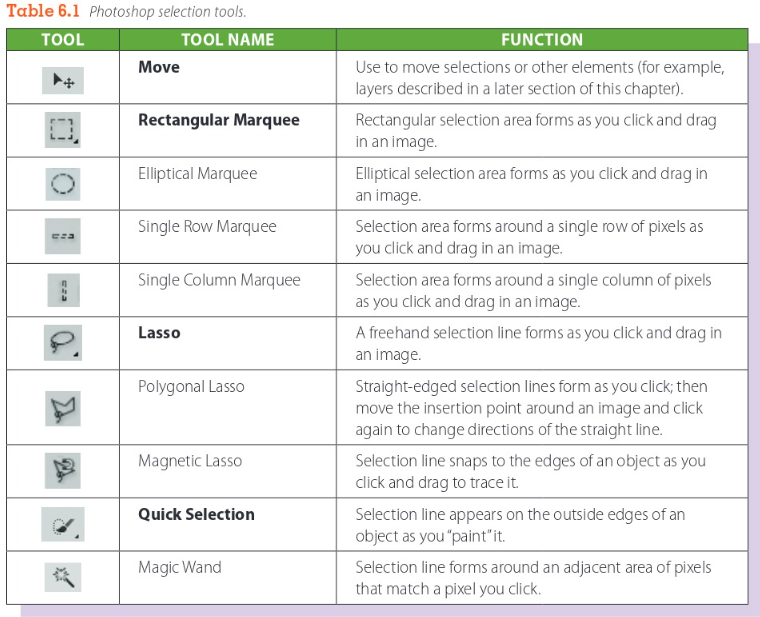
\includegraphics[scale=0.5]{1.png}
    \end{center}
    \bigbreak \noindent 
    Making a selection with one of the marquee tools like the Rectan-gular or Elliptical Marquee tool is easy if the area you want to select is a clearly defined shape. You simply click the tool and then click and drag around the item you wish to select.However, choosing just the pixels you want to work with in an irregularly shaped item can be more challenging. For these areas of image, you can use the Lasso tool to draw freehand around the item you want to select
    \bigbreak \noindent 
    \nt{If you want to be more precise, you can make your selection using the Magic Wand, Magnetic Lasso, or Quick Selection tools. These tools detect where colors in an image begin to change and use that information to establish a selection line.}
    
    \bigbreak \noindent \bigbreak \noindent 
    \begin{Large}
      \textbf{Selection Settings:}
    \end{Large}
    
    \bigbreak \noindent 
    As mentioned earlier in this chapter, when you click a tool, the Control panel toward the top of the Photoshop window displays settings for that particular tool. It is impractical to describe all of the various set-tings in this book, but because some of these settings appear in many different raster programs, it may be helpful to learn what a few of these options mean as you begin learning about image editing.

    \bigbreak \noindent \bigbreak \noindent 
    \begin{large}
      \textbf{Anti-Aliasing and Feathering:}
    \end{large}
    \bigbreak \noindent 
    Because bitmap images are created using square pixels, the edges of a selection can be ragged when you make a selection with a curved line. This is particularly problematic when you ultimately cut or copy and paste a selection. To soften the edges of a selection, select the anti-aliasing option. Anti-aliasing works by softening the color of the pixels along the edge of the selection.
    \bigbreak \noindent 
    Feathering is another way to soften harsh edge lines in a selection. Feathering works by creating a border along the edges of a selection that fades gradually into the background (see Figure 6.9). The result is a soft blur at the edges of the selection.
    \bigbreak \noindent 
    \nt{You set the width of the feath-ering effect in pixels.}

    \bigbreak \noindent \bigbreak \noindent 
    \begin{large}
      \textbf{Additional Magic Wand Tool Settings:}
    \end{large}
    \bigbreak \noindent 
    In addition to anti-aliasing, the Magic Wand tool in Photoshop includes a cou-ple of other settings that you may see for similar tools in other raster editing programs. The tolerance setting deter-mines how precisely the Magic Wand tool does its job. The tolerance deter-mines how many pixels are affected when you use the tool. The higher the tolerance, the higher the number of pix-els affected
    \bigbreak \noindent 
    The default tolerance for the Magic Wand tool is 32 pixels. This means that in addition to all of the pixels that match the first pixel you click, the Magic Wand tool will also select any pixels that are 32 shades darker and 32 shades lighter than the original. If you increase the tolerance, more pixels will be included in the selection. If you decrease it, fewer pixels will be included.
    \bigbreak \noindent 
    Another Magic Wand tool setting to consider is the contiguous option. Contiguous refers to pixels that “touch.” If the contiguous setting is selected (indicated with a check mark), only pixels that are touch-ing will be included in the selection when you click an image with the Magic Wand. Any other pixels within the tolerance but not linked to the original pixel selection will not be included in the selection. However, if the contiguous setting is not selected, all pixels within the tolerance will be included in the selection no matter where they appear

    \bigbreak \noindent \bigbreak \noindent 
    \begin{Large}
      \textbf{Quick Mask Mode:}
    \end{Large}
    \bigbreak \noindent 
    Near the bottom of the Tools panel in Photoshop is a rectangular icon with a small circle in the center. When you click this icon, you access a special selection feature called Quick Mask mode. Quick masks are not to be confused with layer masks, which you’ll learn about later in this chapter. Quick masks enable you to make and refine selections using the Brush tool.
    \bigbreak \noindent 
    when you make a selection, you are es-sentially protecting the unselected area of the image from any changes you make to the selected area inside the marching ants. This is called masking. If you make a selection using one of the selection tools and then click the Quick Mask mode icon on the Tools panel, a ruby-colored overlay appears over the entire image
    \bigbreak \noindent
    The ruby area is the mask formed by the selection. To adjust what is covered by the mask, click the Brush tool and paint with black to cover more area with the mask or with white to reveal more area. Click the Quick Mask mode icon again and the marching ants will reveal the selected areas as indicated by an updated selection outline

    \bigbreak \noindent \bigbreak \noindent 
    \begin{Large}
      \textbf{Digital Photos: Fixing Common Problems and Enhancing Images:}
    \end{Large}
    \bigbreak \noindent 
    Sometimes you capture a great image with your digital camera but something just isn’t right. Perhaps it is a little dark or the composition is off. Luckily, raster editing programs offer easy-to-use tools for fixing common problems.

    \bigbreak \noindent \bigbreak \noindent 
    \begin{large}
      \textbf{Adjusting Brightness and Contrast:}
    \end{large}
    \bigbreak \noindent 
    Brightness and contrast in raster images are sometimes referred to in terms of levels. Levels fall into three basic categories: highlights, shad-ows, and midtones. Highlights represent the lightest part of the image; shadows, the darkest; and midtones, the middle range. Adjusting the levels of any of these three areas can dramatically improve a picture.
    \bigbreak \noindent 
    Another simple way to adjust the levels with the curves function is to use eyedroppers like those shown to the left of the graph in Photoshop’s Curves panel (Figure 6.13). Use the black-tipped eyedropper to select the darkest (blackest) point in the image to set as the shadow. Use the white-tipped eyedropper to select the lightest (whitest) color in the image to set the highlights. Use the gray-tipped eyedropper to select and set a midtone.

    \bigbreak \noindent \bigbreak \noindent 
    \begin{large}
      \textbf{Cropping:}
    \end{large}
    \bigbreak \noindent 
    You can easily use the cropping tool in raster editing software to achieve good com-position in your images
    \bigbreak \noindent 
    In Photoshop, the Crop tool automatically lays a rule of thirds grid over the image so that you can crop using those guidelines. The area inside the crop outline is highlighted and the area outside is dimmed. You can adjust the selection area by using the arrow keys on the keyboard or by clicking and dragging the handles on the outline. When you commit the change, the outside area is cropped out of the picture, leaving just the highlighted part of the image.

    \bigbreak \noindent \bigbreak \noindent 
    \begin{large}
      \textbf{Using Retouch Tools:}
    \end{large}
    \bigbreak \noindent 
    Sometimes you’ll want to change the content in your images, perhaps to remove a distracting element or enhance a person’s appearance in a por-trait. Raster editing software features retouch tools that enable you to make changes like these.
    \bigbreak \noindent 

    \bigbreak \noindent \bigbreak \noindent 
    \begin{Large}
      \textbf{Introduction to Layers And Masks:}
    \end{Large}
    \bigbreak \noindent 
    When you first start working with raster editing programs, your tasks may be simple, like making adjustments similar to the changes covered in the previous section. However, as your tasks become more com-plex, you’ll likely begin using more powerful features called layers and masks. The following section is a brief introduction to the concepts of layers and masks
    
    \bigbreak \noindent \bigbreak \noindent 
    \begin{large}
      \textbf{Understanding Layers:}
    \end{large}
    \bigbreak \noindent 
    Layers are often described as a digital version of a stack of clear plastic sheets, where printed material from lower layers is visible through the clear areas of upper layers. In a program that offers the layers feature, each new file—whether you are opening a digital photo file or creating a new raster document—begins with a single layer. You add layers as needed to do the following sorts of things:

    \bigbreak \noindent 
    \begin{itemize}
      \item Combine and overlap multiple images
      \item Draw vector shapes on a raster image
      \item Add text to an image
      \item Change the order of overlapping items (move from front to back or vice versa, for example)
      \item Adjust the position of different elements independently
      \item Apply special effects and filters
    \end{itemize}
    \bigbreak \noindent 
    This is called nondestructive editing because no part of the original image is altered in the process. Nondestructive editing gives you great freedom to experiment and also allows you to create multiple and varied final images from one initial image.

    \bigbreak \noindent \bigbreak \noindent 
    \begin{large}
      \textbf{Background and Normal Layers:}
    \end{large}
    \bigbreak \noindent 
    You manage layers in Photoshop by using the Layers panel, which opens by default along the right side of the Photoshop workspace.
    \bigbreak \noindent 
    As mentioned above, new raster documents in applications with a layers feature begin with a single layer called the background layer.
    \bigbreak \noindent 
    The back-ground layer is a special kind of layer with certain restrictions:
    \bigbreak \noindent 
    \begin{itemize}
      \item It is always the bottom layer no matter how many other layers you add.
      \item It cannot be renamed.
      \item It cannot be transparent.
      \item It cannot be moved or deleted. (Notice the small lock icon next to the Background layer in Figure 6.15. This icon indicates that a layer is locked and cannot be moved or deleted.)
    \end{itemize}
    \bigbreak \noindent 
    These restrictions also apply to objects and changes you make on the background layer. So, for example, if you add a shape, such as an arrow, to an image on the background layer and then want to reposition it using the Move tool, you can’t. The background and its objects are locked. Likewise, if you try to select and delete the arrow using a selection tool such as a marquee tool or the Magic Wand, the selection area will fill with the background color. For maximum flexibility, it’s best to make changes and adjust-ments on a “normal” layer.
    \bigbreak \noindent 
    Also notice the drop-down list at the top left of the Layers panel. This is the Blending Modes menu. Blending modes affect how a layer blends into the layers below it. The default blending mode is Normal as shown in Figure 6.15, but you can achieve many different effects by choosing from the list that appears when you click the list arrows to the right of the option box
    \bigbreak \noindent 
    \nt{Sometimes, you may find it useful to create a new layer by duplicating an existing layer}
    \bigbreak \noindent 

    \pagebreak \bigbreak \noindent
    \begin{large}
      \textbf{Basic Layer Actions:}
    \end{large}
    \bigbreak \noindent 
    \begin{center}
      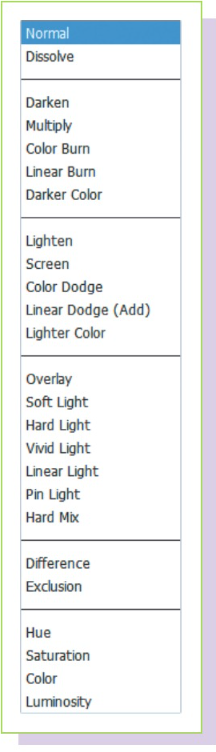
\includegraphics[scale=0.5]{2.png}
    \end{center}

    \bigbreak \noindent \bigbreak \noindent 
    \begin{large}
      \textbf{Layer Styles and Adjustment Layers}
    \end{large}
    \bigbreak \noindent 
    Once you’ve created a new layer, the first thing to do is rename it using a logical and understandable name.
    \bigbreak \noindent 
    Once a layer is created and renamed, you can add color and other details just as you would to any image. You can also take advantage of any shortcuts your raster editing program offers for adding special effects to a layer
    \bigbreak \noindent 
    Styles feature to add special effects to your images. Layer styles are spe-cial effects such as drop shadows and glowing edges that you can add to specific layers in your image.
    \bigbreak \noindent 
    \nt{When you add a layer style, “fx” appears next to the layer name in the Layers panel and the name of the style is indented below}
    \bigbreak \noindent 
    Another nondestructive Photoshop shortcut feature is Adjustment Layers. Adjustment layers allow you to change elements like the light-ing, color, and tones of an image without actually changing the pixels in the original image.
  
    \bigbreak \noindent \bigbreak \noindent 
    \begin{large}
      \textbf{Understanding Layer Masks:}
    \end{large}
    \bigbreak \noindent 
    Recall from earlier in this lesson that you can adjust the transparency of normal layers using the tools on the Layers panel. Layer transparency can vary from completely see-through (0%) to completely solid (100%) and every level in between. Using these tools to adjust layer transpar-ency affects everything on the layer equally
    \bigbreak \noindent 
    But what if you want to adjust the transparency of just a certain part of the layer? In that case, you use something called a mask
    \bigbreak \noindent 
    A layer mask is not too different from a Halloween mask: it hides everything except where holes are cut out. Similarly, a layer mask can hide everything on a layer except what you tell it to reveal. In Photo-shop, you add a mask to a selected layer using the Add layer mask icon (the gray rectangle with a circle in the center on the toolbar at the bottom of the Layers panel). A rectangle appears next to the layer thumbnail in the Layers panel connected by a chain link. This is the layer mask

    \bigbreak \noindent \bigbreak \noindent 
    \begin{large}
      \textbf{Layers, File Size, and File Format}
    \end{large}
    \bigbreak \noindent 
    If you save a layered image in a file format that is native to the image editing software, such as PSD for Photoshop, the layers will remain available to you even after you have closed the file. If you save your image as a JPG or other nonnative file format, the layers will be merged into a single image and you will no longer be able to edit them indi-vidually. However, layers contribute to large file sizes, so the benefit of merging multiple layers into a single layer is a smaller file.
    \bigbreak \noindent 
    Even if you intend to keep your files only in a native format and never save them as a nonnative format such as JPG, you may want to minimize file size for one reason or another. In these cases, you can flatten the image, which merges all of the layers into a single layer and reduces the file size. In Photoshop, you can flatten an image by choos-ing Flatten Image from the Layers menu on the Application bar. How-ever, if you do this, remember that you will no longer be able to adjust individual layers, so it is good to develop the habit of saving a copy of a file before flattening it


\end{document}
